\begin{frame}{Geometric and topological computing}
\protect\hypertarget{geometric-and-topological-computing}{}

\framesubtitle{rethinking some foundations}

\begin{columns}[T]
\begin{column}{0.48\textwidth}
Complexity of geometric information stems from dramatic increase in
\emph{size}, \emph{diversity}, and \emph{complexity} of
\textbf{geometric data}:

\begin{itemize}
% \tightlist
\item
  point clouds,
\item
  boundary meshes,
\item
  NURBs representations,
\item
  finite element meshes,
\item
  CT scans,
\item
  and so on
\end{itemize}
\end{column}

\begin{column}{0.48\textwidth}
Emerging applications (e.g. \textbf{medical 3D}) require the
\textbf{convergence of data structures} from:

\begin{itemize}
% \tightlist
\item
  3d computer imaging
\item
  computer graphics
\item
  solid modeling
\item
  computer-aided geometric design
\item
  discrete meshing of domains
\item
  physical simulations
\end{itemize}
\end{column}
\end{columns}

The goals of \emph{unification}, \emph{scalability}, and
\emph{distributed computing} call for \emph{rethinking some foundations}
of geometric and topological computing

\end{frame}

% \begin{withoutheadline}
    \begin{frame}[plain]{Motivation for a new start}
    \protect\hypertarget{motivation-for-a-new-start}{}
    
    \begin{columns}[T]
    \begin{column}{0.48\textwidth}
    % \begin{block}
    {\small Quad-edge data structure \cite{Guibas1985}}
    
    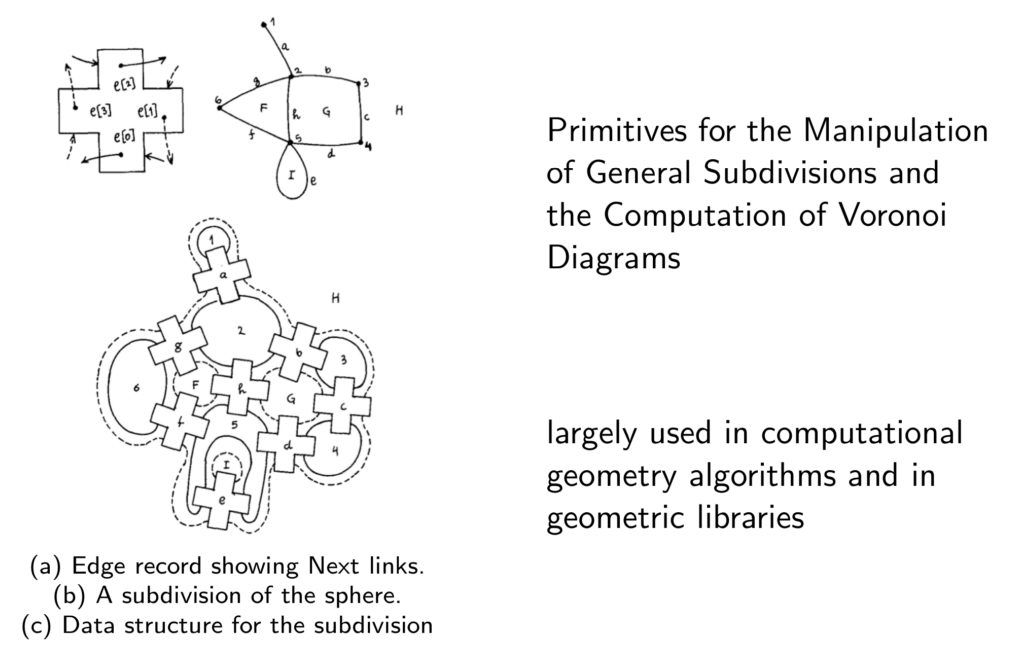
\includegraphics[width=0.98\textwidth]{figs/Guibas1985_quad_edge.png}~
    
    % \end{block}
    
    % \begin{block}
    {\small Hybrid Edge data sturcture \cite{Kalay1989}}
    
    { \scriptsize
    a topological data structure for vertically integrated geometric
    modelling
    
    }
    
    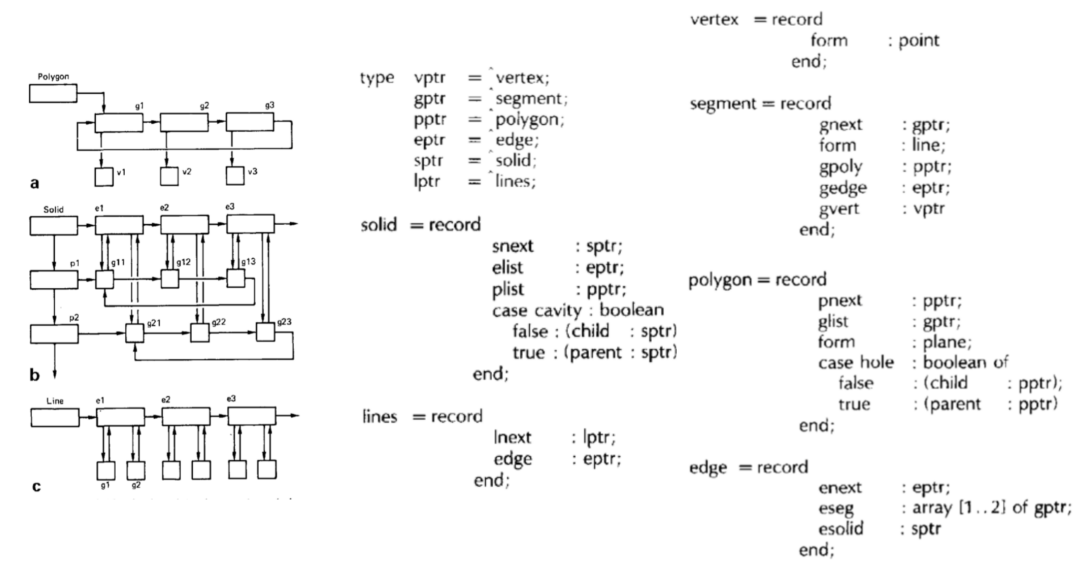
\includegraphics[width=0.98\textwidth]{figs/Kalay1989_hybrid_edge.png}~
    
    % \end{block}
    \end{column}
    
    \begin{column}{0.48\textwidth}
    % \begin{block}
    {\small Partial-Entity data structure \cite{SangHunLee2001}}
    
    {\scriptsize
    Compact Non-Manifold Boundary Representation Based on Partial
    Topological Entities
    }
    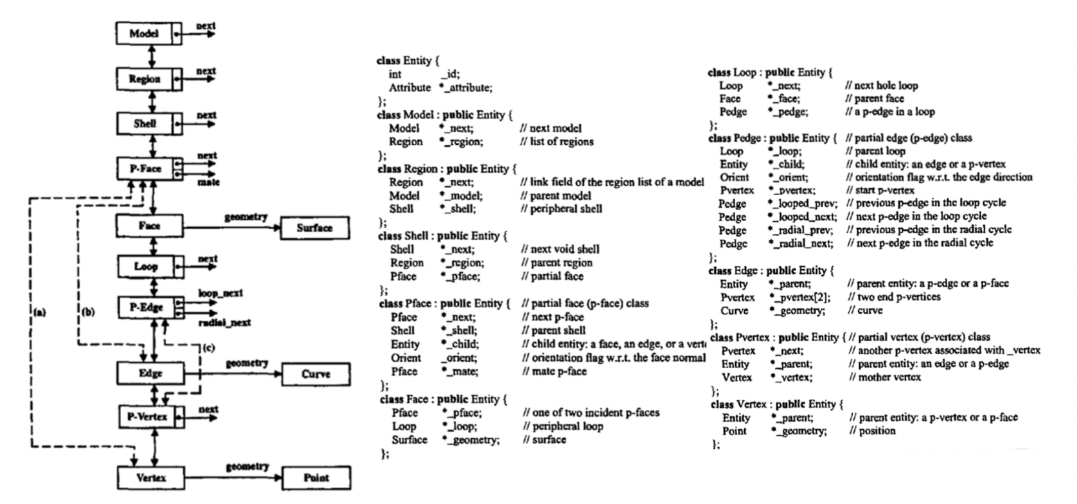
\includegraphics[width=0.98\textwidth]{figs/SangHunLee2001_partial_entity.png}~
    
    % \end{block}
    
    % \begin{block}
    {\small Coupling Entities data structure
    \cite{yamaguchi1995nonmanifold}}
    
    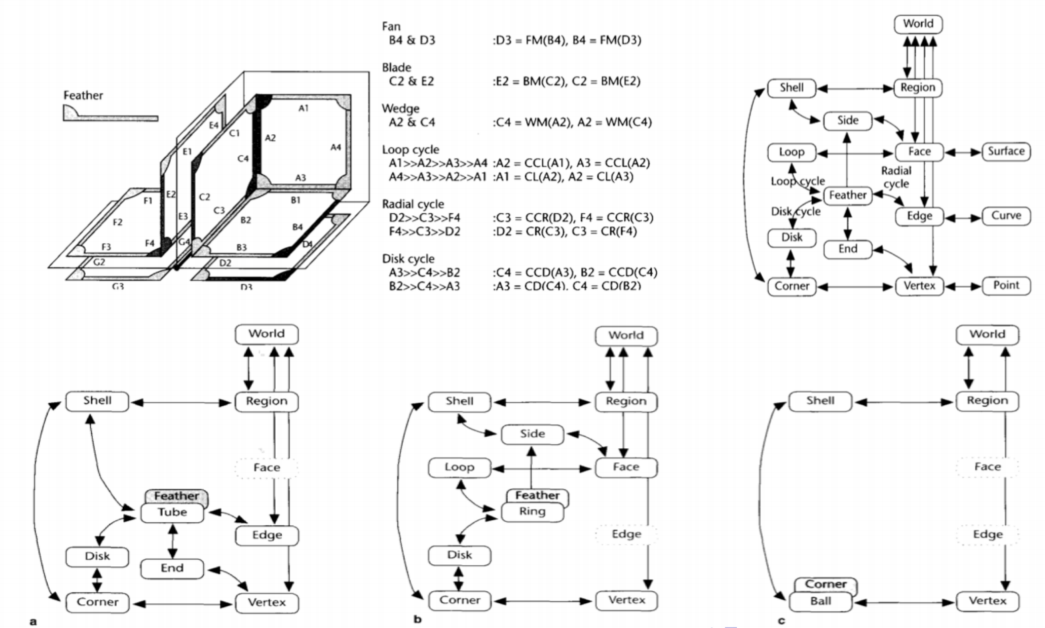
\includegraphics[width=0.98\textwidth]{figs/yamaguchi1995nonmanifold.png}~
    
    % \end{block}
    \end{column}
    \end{columns}
    
    \end{frame}
% \end{withoutheadline}



% \begingroup
% \setbeamertemplate{navigation symbols}{}
% \begin{frame}
% \frametitle{Outline}
% \tableofcontents
% \end{frame}
% \endgroup

% \begin{frame}
% \begin{block}{first sub}



% \begin{itemize}
% % \tightlist
% \item
%   asdf
% \item
%   neks
% \end{itemize}

% \end{block}

% \begin{block}{second sub}

% \begin{itemize}
% % \tightlist
% \item
%   asf
% \item
%   woens
% \end{itemize}

% \end{block}

% \end{frame}

% \begin{frame}{third slide}
% \protect\hypertarget{third-slide}{}

% asdfa sd asd fas

% \end{frame}

% \begin{frame}{My slide}
% \protect\hypertarget{my-slide}{}

% \begin{block}{First column}

% contents

% \end{block}

% \begin{block}{Second column}

% contents

% \end{block}

% \end{frame}
